\documentclass{tikzposter}
\usepackage{jgu_tikzposter}

\title{Retention Time Alignment}
\institute{University Medical Center, Johannes Gutenberg University, Germany}
\author{Mateusz Krzysztof Łącki, Ute Distler, Stefan Tenzer}
\insertlogo[width=10cm]{img/jgu3.pdf}
\insertqr[3in]{https://github.com/MatteoLacki/rta}

\begin{document}
\maketitle

\begin{columns}
\column{0.5}


\block{Rationale}{
	\begin{itemize}
		\good LC-IM-MS instruments identify thousands of peptides obtained from digested proteins
		\bad most observed signals are not easily sequenced and are useless in the identification process
		\good one can retrieve a lot of unidentified signals by x-annotation!
	\end{itemize}
	\begin{tikzfigure}
		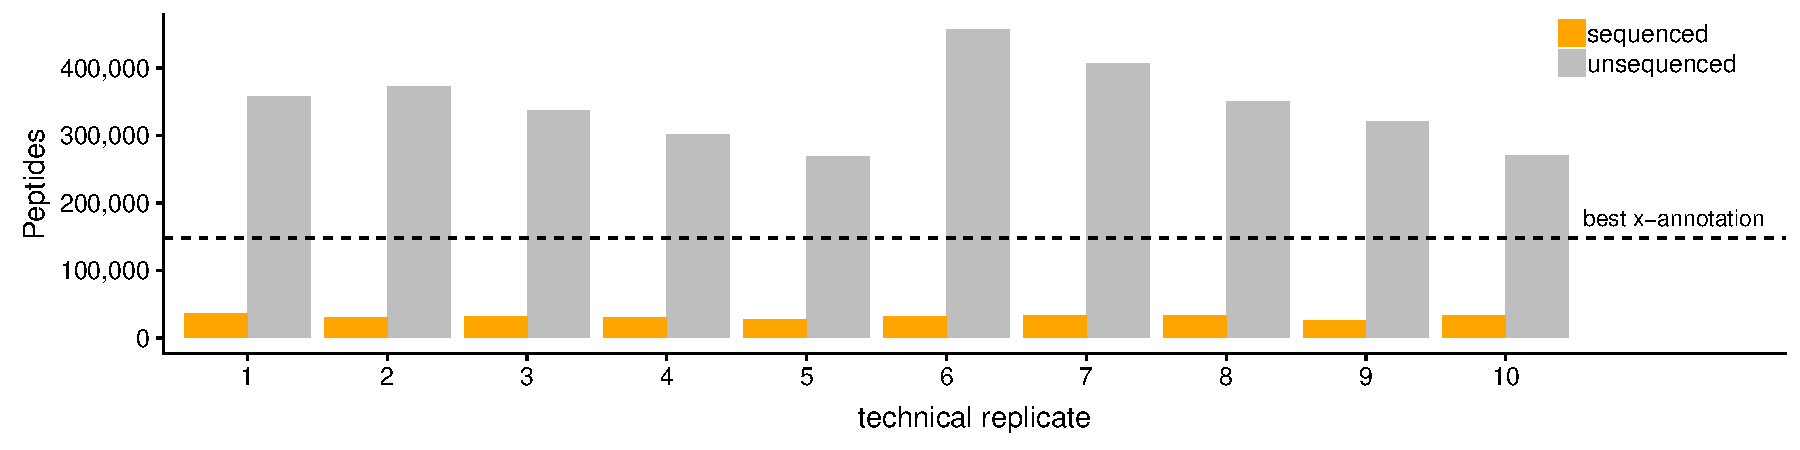
\includegraphics[width=\linewidth]{R/img/x-annotation.pdf}
	\end{tikzfigure}

	\begin{itemize}
		\ugly technical replicates reveal not always the same peptides
		\good biochemical properties of signals in different runs are similar
	\end{itemize}
	
	\begin{tikzfigure}
		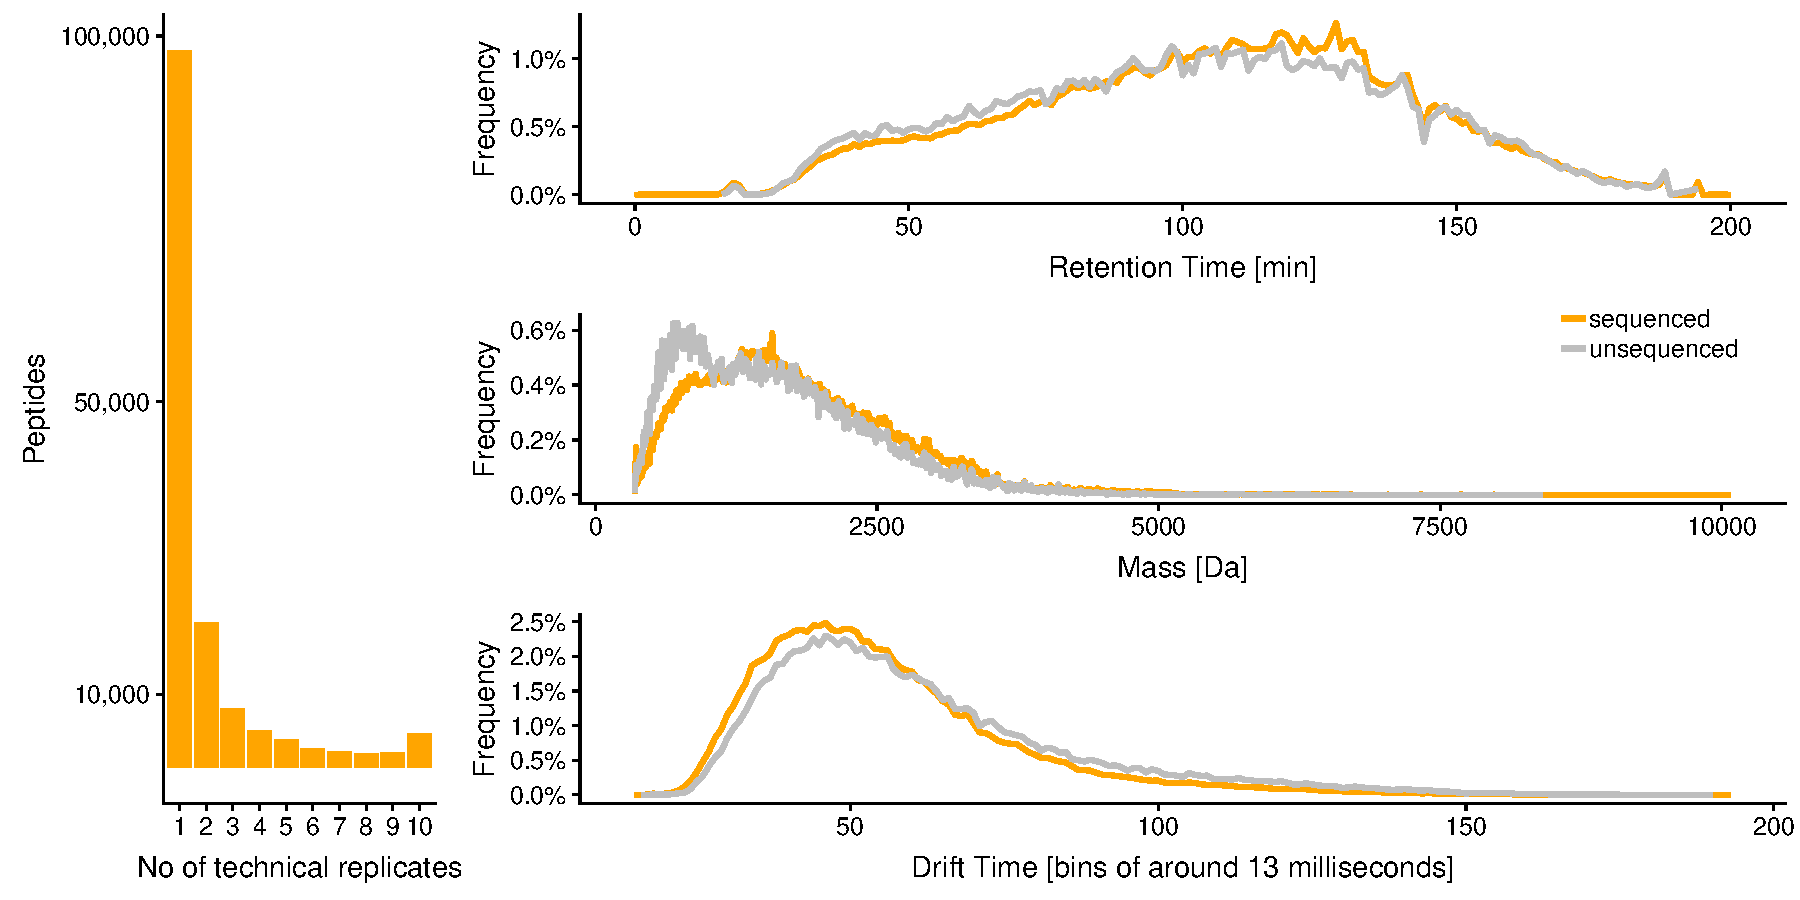
\includegraphics[width=\linewidth]{R/img/venn_and_similarfeatures.pdf}
	\end{tikzfigure}

	\begin{itemize}
		\bad retention times accross technical replicates do show significant systematic deviations
		\bad some sequenced peptides differ significantly between runs (mostly by few minutes)
	\end{itemize}

	\begin{tikzfigure}
		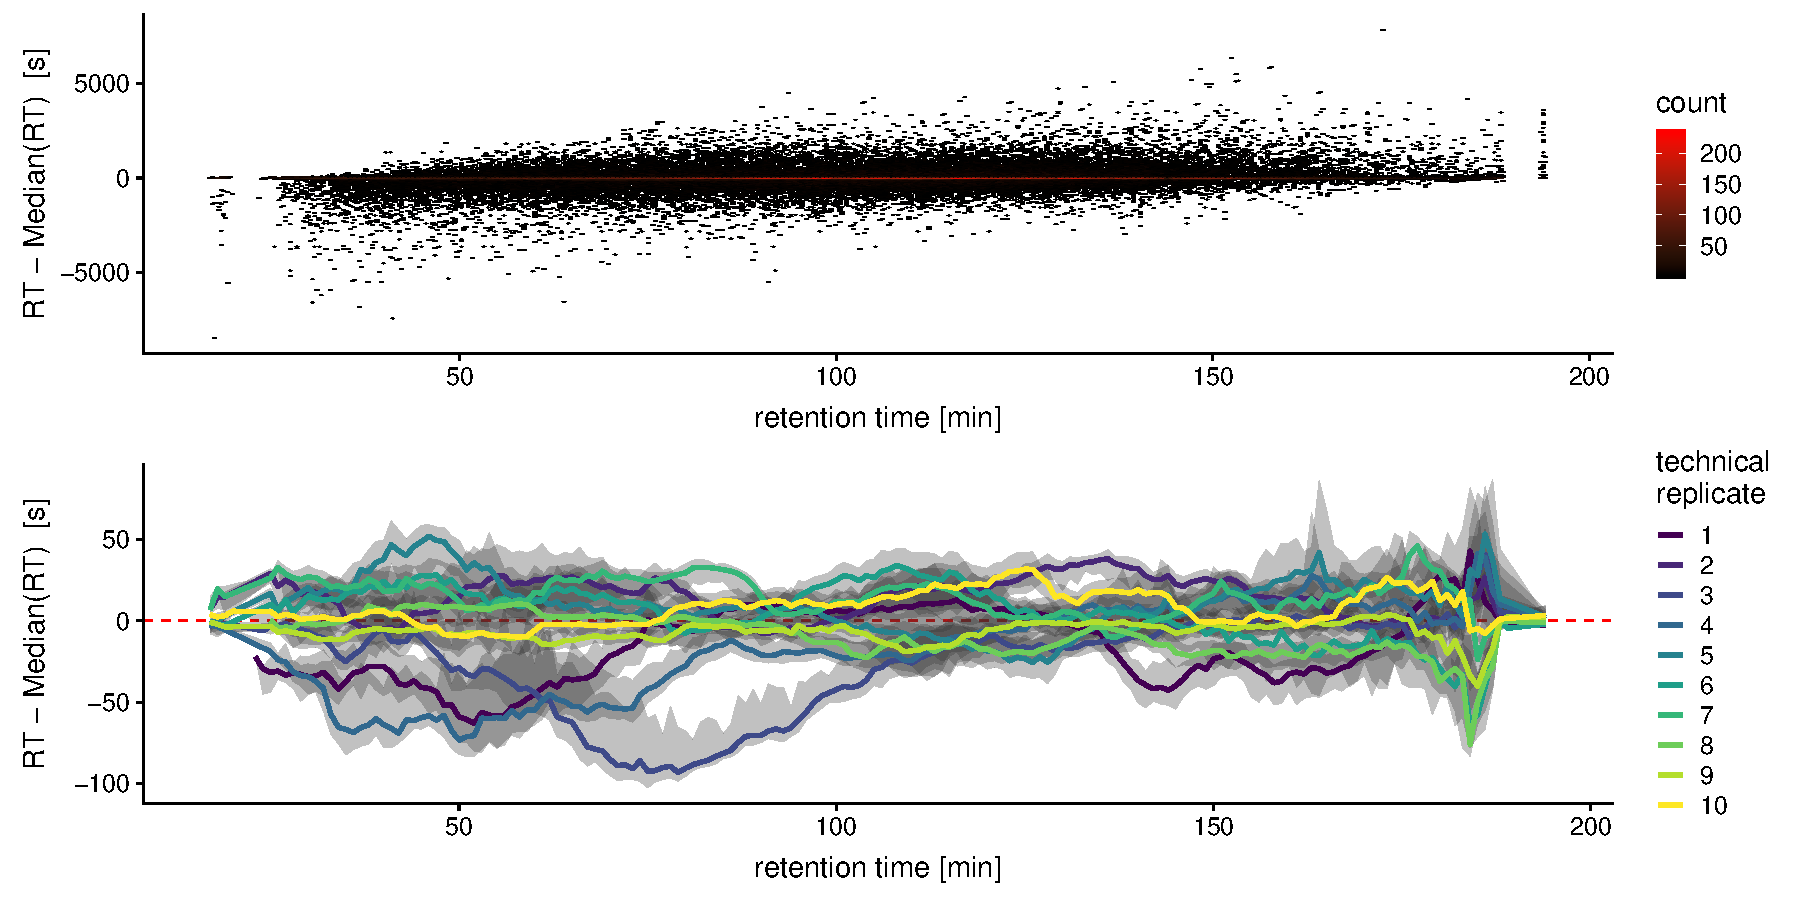
\includegraphics[width=\linewidth]{R/img/rt_dists.pdf}
	\end{tikzfigure}
} 

\block{Retention Time Alignment to the rescue}{
	Brag about the RTA.
}



\column{0.5}


\block{Other similar approaches}{
	The idea of the retention times alignment is not new.
	The \texttt{Match Between Runs} has been a standard part of the \texttt{Max Quant} software\cite{tyanova2016maxquant}.
}

\block{Literature}{
	\bibliographystyle{plain}
	\bibliography{bib/spectrometry}
}
\end{columns}

%\note{Notetext} % See Section 4.3
\end{document}
